\documentclass[]{report}
% http://www.tug.dk/FontCatalogue/charter/
%\usepackage[bitstream-charter,sfscaled=false]{mathdesign}
\usepackage[T1]{fontenc}
%\usepackage{lmodern}
\usepackage{amsmath}
%\usepackage{amssymb}
\usepackage{ifxetex,ifluatex}
\usepackage{fixltx2e} % provides \textsubscript
% use upquote if available, for straight quotes in verbatim environments
\IfFileExists{upquote.sty}{\usepackage{upquote}}{}
\ifnum 0\ifxetex 1\fi\ifluatex 1\fi=0 % if pdftex
  \usepackage[utf8]{inputenc}
\else % if luatex or xelatex
  \ifxetex
    \usepackage{mathspec}
    \usepackage{xltxtra,xunicode}
	 \usepackage{titlesec}
    \setmainfont[Ligatures=TeX]{Charis SIL}
    \newfontfamily\rmfontsc[Ligatures=TeX]{Charis SIL Bold:+smcp}
    \setsansfont[Ligatures=TeX]{FreeSans}
    \setmonofont[Scale=MatchLowercase]{Source Code Pro}

    \titleformat*{\section}{\LARGE\bfseries\sffamily}
    \titleformat*{\subsection}{\large\scshape\rmfontsc}
    \titleformat*{\subsubsection}{\scshape\rmfontsc}

  \else
    \usepackage{fontspec}
  \fi
  \defaultfontfeatures{Mapping=tex-text,Scale=MatchLowercase}
  \newcommand{\euro}{€}
\fi
% use microtype if available
\IfFileExists{microtype.sty}{\usepackage{microtype}}{}
\usepackage{setspace}
\usepackage{xcolor}

\usepackage{caption}
\DeclareCaptionFormat{lstcaption}{\small\itshape #1#2#3}
% below is the general caption setup
% \captionsetup{format=lstcaption}
\captionsetup[lstlisting]{position=bottom,format=lstcaption}

\usepackage{listings}
\lstset{
  basicstyle=\ttfamily,
  xleftmargin=\parindent,
  breaklines=true,
  extendedchars=true,
  tabsize=2,
  keywordstyle=\bfseries\color{green!40!black},
  commentstyle=\itshape\color{purple!40!black},
  identifierstyle=\color{black},
  stringstyle=\color{orange}
}

\lstdefinestyle{c}{
  basicstyle=\footnotesize\ttfamily,
  belowcaptionskip=1\baselineskip,
  numbers=left,
  numbersep=10pt, % how far the line-numbers are from the code
  numberstyle=\ttfamily,
  frame=single,
  language=C,
  showstringspaces=false,
  captionpos=b
}

\lstdefinestyle{code}{
  basicstyle=\footnotesize\ttfamily,
  belowcaptionskip=1\baselineskip,
  numbers=left,
  numbersep=10pt, % how far the line-numbers are from the code
  numberstyle=\ttfamily,
  frame=single,
  showstringspaces=false,
  captionpos=b
}

\lstdefinestyle{simple}{
  belowcaptionskip=1\baselineskip,
  basicstyle=\footnotesize\ttfamily,
  aboveskip=1\baselineskip,
  belowskip=1\baselineskip,
  xleftmargin=5mm,
  % language=TeX,
  showstringspaces=false,
  numbers=none,
  frame=none,
  keywordstyle=\bfseries\color{green!40!black},
  commentstyle=\itshape\color{purple!40!black},
  identifierstyle=\color{black},
  stringstyle=\color{orange},
  captionpos=b
}
\usepackage{fancyvrb}
\usepackage{longtable,booktabs}
\usepackage{graphicx}
% Redefine \includegraphics so that, unless explicit options are
% given, the image width will not exceed the width of the page.
% Images get their normal width if they fit onto the page, but
% are scaled down if they would overflow the margins.
\makeatletter
\def\ScaleIfNeeded{%
  \ifdim\Gin@nat@width>\linewidth
    \linewidth
  \else
    \Gin@nat@width
  \fi
}
\makeatother
\let\Oldincludegraphics\includegraphics
{%
 \catcode`\@=11\relax%
 \gdef\includegraphics{\@ifnextchar[{\Oldincludegraphics}{\Oldincludegraphics[width=\ScaleIfNeeded]}}%
}%
\ifxetex
  \usepackage[setpagesize=false, % page size defined by xetex
              unicode=false, % unicode breaks when used with xetex
              xetex]{hyperref}
\else
  \usepackage[unicode=true]{hyperref}
\fi
\hypersetup{breaklinks=true,
            bookmarks=true,
            pdfauthor={},
            pdftitle={Energy-aware virtual CPU scheduler},
            colorlinks=true,
            citecolor=blue,
            urlcolor=blue,
            linkcolor=magenta,
            pdfborder={0 0 0}}
\urlstyle{same}  % don't use monospace font for urls
\setlength{\parindent}{0pt}
\setlength{\parskip}{6pt plus 2pt minus 1pt}
\setlength{\emergencystretch}{3em}  % prevent overfull lines
\setcounter{secnumdepth}{0}
\VerbatimFootnotes % allows verbatim text in footnotes

\title{Energy-aware virtual CPU scheduler}
\author{}


\begin{document}
\maketitle

{
\hypersetup{linkcolor=black}
\setcounter{tocdepth}{2}
\tableofcontents
}
\chapter{Introduction}\label{introduction}

\emph{Written by Andrii Berezovskyi \& Armand Zangue}

\section{Scope}\label{scope}

This is a documentation for the scheduler developed as part of the
project on Operating Systems at KBS. The main purpose of the scheduler
is to save power on a server mainly used to run virtual machines. The VM
hypervisor for this project is QEMU\footnote{Which, in turn, relies on
  KVM for acceleration and SMP support using options
  \lstinline!-enable-kvm! and \lstinline!-smp <n>! respectively}.

The remaining part of the document is structured as follows: first, the
scheduler design is described. Then the detailed design of the scheduler
subsystem is given, followed by the documentation of the power-saving
subsystem. Finally, instructions on how to build, install and debug as
well as evualuate the developed project are provided.

\section{Overview}\label{overview}

To achieve the project purpose, the CPU is allocated to virtual machine
CPUs (VCPUs) in superperiods of a fixed duration of 200ms, so that each
VCPU has a certain time to run proportionally to its predefined share of
the CPU. Before the end of each superperiod, if there is any time left,
it can be used to actually save energy.

Linux has a modular scheduler architecture that allows different
scheduling policies to co-exist. These policies are wrapped up in
so-called scheduler classes. Thus, implementing a new scheduling policy
for Linux mainly consists of writing a new scheduler class.

Originally, there are 2 main scheduling classes: Real-Time and
Completely Fair Scheduler (CFS). The Real-Time scheduling class is
responsible for the following policies:

\begin{itemize}
\itemsep1pt\parskip0pt\parsep0pt
\item
  \lstinline!SCHED_FIFO!
\item
  \lstinline!SCHED_RR!
\end{itemize}

The CFS scheduler, on another hand is providing other 2 policies:

\begin{itemize}
\itemsep1pt\parskip0pt\parsep0pt
\item
  \lstinline!SCHED_NORMAL!
\item
  \lstinline!SCHED_BATCH!
\end{itemize}

By default, newly created processes are assigned the \emph{normal}
scheduling policy and all forked subprocesses will inherit it\footnote{Both
  policy and inheritance can be changed via the
  \lstinline!sched_setscheduler(2)! call.}.

Existing schedulers serve their purpose fairly well, robustly scheduling
the tasks while meeting the deadlines and distributing the machine
resources. However, when the system is frequently remaining idle, the
power is not saved or the saving is enable only via the
\textbf{\lstinline!ondemand! in-kernel governor} \footnote{See
  https://www.kernel.org/doc/ols/2006/ols2006v2-pages-223-238.pdf for
  details} or through the \textbf{dynamic frequency scaling} techniques,
such as \emph{Intel SpeedStep} and \emph{Intel Turbo Boost}.

This way, when there are no tasks in the system ready for the execution,
the control is relinquished to the \emph{idle} task.

The idle task basically halts the processor (for \emph{x86}
architecture):

\begin{lstlisting}[style=c, caption=arch/x86/include/asm/irqflags.h, firstnumber=52]
static inline void native_halt(void)
{
  asm volatile("hlt": : :"memory");
}
\end{lstlisting}

This does not yield significant power savings alone, even when combined
with the aforementioned techniques.

\subsubsection{Notice}\label{notice}

The line numbering corresponds to the codebase state as of commit
\href{https://gitlab.tubit.tu-berlin.de/mirko/operating-system-\%20project/tree/9125134e9dcbcdd7a6ce3300712834c6369cfc3b}{9125134e}.
In case of discrepancies, check out the repository at the given commit
hash.

\chapter{Scheduler}\label{scheduler}

\emph{Written by Andrii Berezovskyi, Armand Zangue \& Tamilselvan
Shanmugam}

\section{Integration into the kernel}\label{integration-into-the-kernel}

The scheduler was integrated into the kernel scheduling subsystem by
making changes in the following places.

\subsection{Data structures}\label{data-structures}

The OSPJ scheduler has introduced several changes to the data
structures, mainly located in two \lstinline!sched.h! files\footnote{\lstinline!kernel/sched/sched.h!
  and \lstinline!include/linux/sched.h!}.

First, the \lstinline!'struct ospj_rq'! was defined:

\begin{lstlisting}[style=c, caption=kernel/sched/sched.h, firstnumber=365]
struct ospj_rq {
    struct list_head ospj_list_head;
    struct list_head *ptr_eligible_q;
    struct list_head *ptr_waiting_q;
    struct list_head eligible_q;
    struct list_head waiting_q;
    struct rq *rq;
    struct task_struct *idle;
    unsigned int nr_running;
    unsigned int idle_request;
    unsigned int period_ticks;
};
\end{lstlisting}

Main point of interest is the existence of two queues,
\lstinline!eligible_q! and \lstinline!waiting_q!. The meaning of both
queues will be explained below. Another interesting components are the
queue pointers also defined in the structure. They are specifically
defined for easy process of swapping the queues (also explained later).
The runqueue is designed to hold all the tasks assigned to the
responsible scheduling class on one processor. Each CPU has its own
runqueue, which holds the runqueue stuctures for each scheduling class:

\begin{lstlisting}[style=c, caption=kernel/sched/sched.h, firstnumber=413]
/*
 * This is the main, per-CPU runqueue data structure.
 * ...
 */
struct rq {
    ...
    struct cfs_rq cfs;
    struct rt_rq rt;
#ifdef CONFIG_SCHED_VMS
    struct ospj_rq ospj;
#endif /* CONFIG_SCHED_VMS */
    ...
}
\end{lstlisting}

Finally, the scheduling class is defined on a per-task basis:

\begin{lstlisting}[style=c, caption=include/linux/sched.h, firstnumber=1055]
struct task_struct {
    ...
    const struct sched_class *sched_class;
    ...
#ifdef CONFIG_SCHED_VMS
    struct sched_vms_entity vms;
    struct list_head ospj_list_node; /* list item to insert task into Q */
    unsigned int share;
    unsigned int ospj_time_slice;
    unsigned int ospj_assigned_time_slice;
#endif /* CONFIG_SCHED_VMS */
    ...
    unsigned int policy;
\end{lstlisting}

In order to understand how the \lstinline!sched_class! is set, we need
to look into the scheduler hierarchy.

\subsection{Scheduler hierarchy}\label{scheduler-hierarchy}

In order to register a scheduler in a kernel, one must provide a
structure initialized with the pointers to the scheduler functions.
Below you can find the excerpt of the structure defined for our
scheduler:

\begin{lstlisting}[style=c, caption=ospj.c, firstnumber=556]
const struct sched_class ospj_sched_class = {
    .next               = &idle_sched_class,
    .enqueue_task       = enqueue_task_ospj,
    .dequeue_task       = dequeue_task_ospj,
    .yield_task         = yield_task_ospj,

    .check_preempt_curr = check_preempt_curr_ospj,

    .pick_next_task     = pick_next_task_ospj,

...

};
\end{lstlisting}

This allows the scheduler subsystem (implemented mainly in
\lstinline!core.c!) to perform generic calls to every scheduler,
e.g.~the following snippet from the \lstinline!pick_next_task! function:

\begin{lstlisting}[style=c, caption=core.c, firstnumber=2949]
for_each_class(class) {
    p = class->pick_next_task(rq);
    if (p)
        return p;
}
\end{lstlisting}

However, before the function of our new scheduling class is going to be
called in this manner, we have to put a pointer to our
\lstinline!struct sched_class! structure into the linked list that is
being iterated in this \lstinline!for! loop. The head of this list is
defined in \lstinline!sched.h!\footnote{there is also defined another
  header under \lstinline!include/linux/sched.h!}:

\begin{lstlisting}[style=c, caption=kernel/sched/sched.h, firstnumber=1041]
#define sched_class_highest (&stop_sched_class)
\end{lstlisting}

Then, each next node of the list is defined in the \lstinline!next!
field of the \lstinline!struct sched_class! structure:

\begin{lstlisting}[style=c, caption=Designated initializer in kernel/sched/sched.h, firstnumber=105]
const struct sched_class stop_sched_class = {
    .next           = &rt_sched_class,
    ...
}
\end{lstlisting}

The original hierarchy is ordered as follows:

\begin{enumerate}
\def\labelenumi{\arabic{enumi}.}
\itemsep1pt\parskip0pt\parsep0pt
\item
  Stop scheduler class.
\item
  RT scheduler class.
\item
  Fair scheduler class.
\item
  Idle scheduler class.
\end{enumerate}

Our implementation inserts a new scheduler class after the fair
scheduler right before the idle class:

\begin{lstlisting}[style=c, caption=fair.c, firstnumber=6167]
const struct sched_class fair_sched_class = {
#ifdef CONFIG_SCHED_VMS
    .next           = &ospj_sched_class,
#else
    .next           = &idle_sched_class,
#endif /* CONFIG_SCHED_VMS */
}
\end{lstlisting}

\subsection{Configuration flags}\label{configuration-flags}

As you can see, the ``insertion'' is done conditionally, depending on
whether the kernel was configured with \lstinline!CONFIG_SCHED_VMS!
flag.

The kernel flag itself is defined in the \lstinline!Kconfig! file:

\begin{lstlisting}[style=c, caption=/Kernel/arch/x86/Kconfig, firstnumber=2334]
menu "VMS scheduler (OSPJ)"

config SCHED_VMS
    bool "Virtual Machines Scheduling (VMS) policy"
    default y
endmenu

}
\end{lstlisting}

This flag is also used to link project-related object files at the later
build stage:

\begin{lstlisting}[style=c, caption=/Kernel/kernel/sched/Makefile, firstnumber=20]
obj-$(CONFIG_SCHED_VMS) += ospj.o
obj-$(CONFIG_SCHED_VMS) += ospj_green_peace.o
\end{lstlisting}

\subsection{Changing scheduling policy to
SCHED\_VMS}\label{changing-scheduling-policy-to-schedux5fvms}

The purpose of \lstinline!sched_setscheduler! syscall is to change the
scheduling policy of given \lstinline!pid! to \lstinline!SCHED_VMS!.

The OSPJ policy defines a new property of process \emph{share} that has
to be passed to the syscall. For this purpose, the
\lstinline!sched_param! structure was also modified:

\begin{lstlisting}[style=c, caption=include/linux/sched.h, firstnumber=7]
struct sched_param {
    int sched_priority;

#ifdef CONFIG_SCHED_VMS
    unsigned int share;
#endif /* CONFIG_SCHED_VMS */
};
\end{lstlisting}

This modified syscall verifies following parameters before changing the
policy:

\begin{enumerate}
\def\labelenumi{\arabic{enumi}.}
\itemsep1pt\parskip0pt\parsep0pt
\item
  Policy should be valid or recognized by the scheduler.
\item
  Priority of the policy should be valid. In \lstinline!SCHED_VMS! case,
  valid priority is \lstinline!0!.
\item
  User should have appropriate permission to change the scheduling
  policy.
\item
  Valid share (1 to 100) must be given.
\end{enumerate}

If all the conditions are satisfied, the scheduling policy of process
\lstinline!pid! can be successfully changed to \lstinline!SCHED_VMS!.

\section{Design and implementation}\label{design-and-implementation}

\subsection{Queues}\label{queues}

The scheduling class performs periodic scheduling using 2 FIFO queues.
There is a need for 2 queues to be in place for implementing a no-return
policy for the tasks that have finished their allotted time (or,
depending on the scheduling mode, those that yielded their priority
before running out of time).

This way, each task which is determined not be allowed to return to the
main \lstinline!eligible_q! queue, are put into the
\lstinline!waiting_q! instead. The queues are eventually swapped, as
outlined later in this section under \textbf{Queue operations}
subsection.

\subsection{Time allocation}\label{time-allocation}

Each VCPU has a time slice within a superperiod computed according to
the share passed in the \lstinline!sched_setscheduler! system call. The
time slice\footnote{One time slice is equal to 10ms} itself is then
calculated by calling the \lstinline!ospj_calc_time_slice! function:

\begin{lstlisting}[style=c, firstnumber=3890, caption=core.c]
__setscheduler_vms(struct rq *rq, struct task_struct *p, int policy, int share)
{
    if(policy == SCHED_VMS && share > 0 && share <= 100) {
        p->sched_class = &ospj_sched_class;
        p->policy = policy;
        p->share = share;
        p->prio = 0;

        ospj_calc_time_slice(p, share);
    ...
\end{lstlisting}

On each call of the \lstinline!task_tick_ospj!, the task time slice is
decremented. When the time slice reaches 0, it is replenished
immediately and the task is forcibly rescheduled:

\begin{lstlisting}[style=c, firstnumber=357, caption=ospj.c]
if (--p->ospj_time_slice == 0) {
        ...
        p->ospj_time_slice = p->ospj_assigned_time_slice;
        set_tsk_need_resched(p);
        yield_task_ospj(rq);
        return;
    }
\end{lstlisting}

\subsection{Task rescheduling}\label{task-rescheduling}

When the task is rescheduled, it is moved from the
\lstinline!eligible_q! to the \lstinline!waiting_q!:

\begin{lstlisting}[style=c, firstnumber=174, caption=ospj.c]
static void requeue_task_ospj(struct rq *rq, struct task_struct *p)
{
    list_move_tail(&p->ospj_list_node, rq->ospj.ptr_waiting_q);
    dprintk(KERN_DEBUG, "[OSPJ] requeue(): del %d, n = %d\n",
           p->pid, rq->ospj.nr_running );
}
\end{lstlisting}

Next task is picked by the \lstinline!pick_next_task_ospj! function.
Generally, during the non-idle period, the next task is picked from the
\lstinline!eligible_q!:

\begin{lstlisting}[style=c, firstnumber=283, caption=ospj.c]
next = list_entry(rq->ospj.ptr_eligible_q->next, struct task_struct, ospj_list_node);
next->se.exec_start = rq->clock_task;
\end{lstlisting}

Otherwise, the \emph{idle} period lasts until the end of the
superperiod.

\subsection{Idle period}\label{idle-period}

After the \emph{eligible} tasks have been scheduled in current
superperiod, it is checked if there is any time left. In case of
success, the ownership of the idle task is taken in the
\lstinline!pick_next_task_ospj! (see \lstinline!ospj.c:244!).

During this period, the power code is supposed to be run instead of
simply halting the processor. During this phase, the OSPJ scheduler is
receiving task tick calls while the idle task is executing.

After the last tick, the scheduling class of the idle task is set back
to \lstinline!idle_sched_class!. This is done in two steps:

\begin{enumerate}
\def\labelenumi{\arabic{enumi}.}
\itemsep1pt\parskip0pt\parsep0pt
\item
  \lstinline!rq->ospj.idle_request! is set to \lstinline!0! in
  \lstinline!task_tick_ospj!.
\item
  Subsequent call to \lstinline!pick_next_task_ospj! results in the
  actual assignment (\lstinline!ospj.c:265!).
\end{enumerate}

\subsection{Superperiod repetition}\label{superperiod-repetition}

Finally, after the superperiod has ended (i.e.
\lstinline!ospj.period_ticks == 0!), the superperiod is replenished and
starts over again with queue swapping.

\subsection{Queue operations}\label{queue-operations}

One of the main operations performed with the queues is \emph{swapping},
which happens in the \lstinline!pick_next_task_ospj! function:

\begin{lstlisting}[style=c, caption=ospj.c, firstnumber=242]
if (is_idle_period(rq)) {
    ...
    /* Swap Qs */
    tmp = rq->ospj.ptr_waiting_q;
    rq->ospj.ptr_waiting_q = rq->ospj.ptr_eligible_q;
    rq->ospj.ptr_eligible_q = tmp;
    d("Queues swaped\n");
}
\end{lstlisting}

As you might see above, it is not the queues itself that are compared,
but their pointers. These pointer fields are initialized in the
\lstinline!init_ospj_rq! call:

\begin{lstlisting}[style=c, caption=ospj.c, firstnumber=63]
ospj_rq->ptr_eligible_q = &ospj_rq->eligible_q;
ospj_rq->ptr_waiting_q = &ospj_rq->waiting_q;

ospj_rq->idle_request = 0;

INIT_LIST_HEAD(&ospj_rq->ospj_list_head);
INIT_LIST_HEAD(ospj_rq->ptr_eligible_q);
INIT_LIST_HEAD(ospj_rq->ptr_waiting_q);
\end{lstlisting}

\section{QEMU threading model}\label{qemu-threading-model}

As our scheduler is primarily targeted at scheduling QEMU threads, it is
worthwhile to discuss its internals that are relevant to the project.

When QEMU is started with 2 virtual CPUs, it creates 3 permanent
threads:

\begin{itemize}
\itemsep1pt\parskip0pt\parsep0pt
\item
  2 threads correspond to 2 VCPUs
\item
  1 thread is responsible for handling IO operations
\end{itemize}

Other threads are temporary/permanent and correspond to any of the
following categories:

\begin{itemize}
\itemsep1pt\parskip0pt\parsep0pt
\item
  Configuration dependent threads
\item
  Worker threads
\item
  Dedicated threads
\item
  Reusable threads
\end{itemize}

\textbf{\emph{Configuration dependent threads:}} It depends on the
virtual machine features. E.g.: VNC thread, Gluster/Ceph.

\textbf{\emph{Worker threads:}} Sometimes long-running computations
simply hog the CPU and are difficult to break up into callbacks. In
these cases dedicated worker threads are used to carefully move these
tasks out of core QEMU.

Examples of worker thread users are \lstinline!posix-aio-compat.c!,
\lstinline!ui/vnc-jobs- async.c!. Worker threads perform specialized
tasks and do not execute guest code or process events.

\textbf{\emph{Dedicated threads:}} Dedicated to perform only one task if
the task is active, e.g.~audio processing.

\textbf{\emph{Reusable threads:}} \lstinline!thread-pool.c! generates
reusable threads.

In general threads will have the same CPU affinity as the main
loop/iothread. There are QMP APIs to query the \lstinline!tid!'s of some
threads.

Also, it is possible to interact with QEMU via the QMP interface. As
this interaction was not viable from kernel-space, this option was
abandoned. Sample code is provided in \textbf{Appendix A}. Also, links
to useful resources are provided at the end of the chapter.

\section{Scheduler evaluation}\label{scheduler-evaluation}

In order to test how well the scheduling subsystem performs, performance
measurements were taken using the Fibonacci element calculation program.

The measurements were performed at each frequency step with the
following configurations (5 times for each configuration to produce a
statistically significant result):

\begin{itemize}
\itemsep1pt\parskip0pt\parsep0pt
\item
  CFS scheduler
\item
  VMS scheduler with 50\% share
\end{itemize}

The results show that the calculation is done in very similar time,
while VMS scheduler showing better results in 2 measurements and CFS -
in 2 others (especially taking into account that the difference in terms
of performance is comparable to the standard deviation within the series
of a single measurement):

\begin{figure}[htbp]
\centering
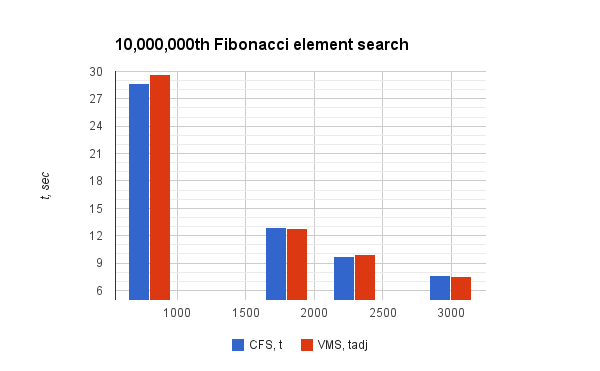
\includegraphics{img/sched_measurement.png}
\end{figure}

The table with the full measurement data is supplied separately.

\section{Useful resources}\label{useful-resources}

\subsection{Scheduler}\label{scheduler-1}

\begin{itemize}
\itemsep1pt\parskip0pt\parsep0pt
\item
  \url{http://wiki.xen.org/wiki/Credit_Scheduler}
\item
  \url{http://www.embedded.com/design/operating-systems/4204929/Real-Time-Linux-Scheduling-Part-1}
\end{itemize}

\subsection{QEMU}\label{qemu}

\begin{itemize}
\itemsep1pt\parskip0pt\parsep0pt
\item
  \url{http://wiki.qemu.org/QMP}
\item
  \url{http://dachary.org/?p=1474}
\item
  \url{https://rubygems.org/gems/qemu}
\item
  \url{https://rubygems.org/gems/qemu-toolkit}
\item
  \url{https://pypi.python.org/pypi/PyQemu/0.1}
\item
  \url{http://blog.vmsplice.net/2011/03/qemu-internals-overall-architecture-and.html}
\item
  \url{http://comments.gmane.org/gmane.comp.emulators.qemu/135139}
\end{itemize}

\chapter{Power saving subsystem}\label{power-saving-subsystem}

\emph{Written by Lukas Braband \& Marat Timergaliev}

\section{What was done by the energy subgroup during the
project}\label{what-was-done-by-the-energy-subgroup-during-the-project}

Floor\ldots{} In one of the first meetings it was pointed out that the
project task requires some kind of ``energy saving idle process''. This
``energy saving idle process'' would run for the amount of time where
the current hyperperiod is already served completely. So during this
timespan no resources (here CPU), agreed on in an SLA, are needed and
therefore should be switched off ``as deeply as possible''.

\section{Power management. CPU sleeping states
access}\label{power-management.-cpu-sleeping-states-access}

Power management implies dynamic frequency or voltage scaling on the
certain devices based on performance needs. In the scope of power
management in the project, the target goal was saving energy within the
usage of CPU during the system idle time.

The finding of an appropriate way of ``switching off'' the CPU(s) turned
out to be a more difficult and time consuming task than initially
expected. Several ideas and approaches had come up. In this part of the
documentation the investigated approaches are depicted.

\subsection{Sleeping states (C-states)}\label{sleeping-states-c-states}

In order to save power, CPU has been enabled to support low-power mode
states, or in other words c-states (sleeping state).

The basic idea of these modes is to cut the clock signal and power from
idle units inside the CPU. The more units you stop (by cutting the
clock), reduce the voltage or even completely shut down, more energy you
save, but more time is required for the CPU to ``wake up'' and be again
100\% operational.

The CPU power states C0--C3 are defined as follows:

\begin{itemize}
\item
  \textbf{C0} is the operating state.
\item
  \textbf{C1} (often known as Halt) is a state where the processor is
  not executing instructions, but can return to an executing state
  essentially instantaneously. All ACPI-conformant processors must
  support this power state. Some processors, such as the Pentium 4, also
  support an \lstinline!Enhanced C1 state! (\lstinline!C1E! or Enhanced
  Halt State) for lower power consumption.
\item
  \textbf{C2} (often known as Stop-Clock) is a state where the processor
  maintains all software-visible state, but may take longer to wake up.
  This processor state is optional.
\item
  \textbf{C3} (often known as Sleep) is a state where the processor does
  not need to keep its cache coherent, but maintains other state. Some
  processors have variations on the C3 state (Deep Sleep, Deeper Sleep,
  etc.) that differ in how long it takes to wake the processor. This
  processor state is optional.
\end{itemize}

Additional states are defined by manufacturers for some processors. For
example, Intel's Haswell platform has states up to C10, where it
distinguishes core states and package states.

C-states are dynamically requested by software and are exposed through
ACPI objects. C-states can be requested on a per-core basis. Software
requests a C-state change in one of two ways, either by executing the
HLT instruction or, for revision E, by reading from an IO specific
address \lstinline!CstateAddr!.

Since the access to c-states required installed ACPI module, here is the
required configuration for linux in order to enable ACPI.

\begin{lstlisting}[style=simple]
CONFIG_PM=y
CONFIG_ACPI=y
CONFIG_ACPI_AC=y
CONFIG_ACPI_BATTERY=y
CONFIG_ACPI_BUTTON=y
CONFIG_ACPI_FAN=y
CONFIG_ACPI_PROCESSOR=y
CONFIG_ACPI_THERMAL=y
CONFIG_ACPI_BLACKLIRG_YEAR=0
CONFIG_ACPI_EC=y
CONFIG_ACPI_POWER=y
CONFIG_ACPI_SYSTEM=y
\end{lstlisting}

We had written the basic class in order to read the \lstinline!msr!
register, specific for the certain processor. D18f4x118 recommended
\lstinline!msr! register to read, in order to send the CPU core to a
c-state.

The result was not satisfactory, since the system's ACPI was still not
enabled due to the absence of ACPI component on the motherboard.

We applied different techniques to resolve the absence of necessary
component. Various reasons may exist of failing this task which are
related to the different aspects such as lack of knowledge and proper
documentation, CPU or motherboard related problems (may not support it),
absence of necessary drivers for current CPU and etc.

Some work, that has been done in order to investigate possible solution
to enable ACPI and CPU idle states was as follows:

\begin{itemize}
\itemsep1pt\parskip0pt\parsep0pt
\item
  Update BIOS. It had to have a special configuration field to enable or
  disable ACPI, which was absent.
\item
  Installation of \lstinline!powertop! didn't show that the system has
  any cpu idle state.
\item
  Research for possible reason of idle states absence
\item
  CPU idle was not installed along with ACPI
\item
  CPU idle driver missing. Attempt to find a proper driver for our
  processor failed.
\item
  Research why ACPI doesn't work properly. Can be that in new kernel
  version acpi may require special actions, since it should work from
  \lstinline!/proc/acpi! directory, which is deprecated in our kernel
  version, in favor of \lstinline!/sys! directory. CPU idle
  configuration failed.
\end{itemize}

HLT execution cannot be verified since cpu idle states monitoring does
not work.

\subsection{Core disabling}\label{core-disabling}

The first traditional approach of saving energy did not approve its
efficiency, due of some reasons mentioned above, we decided to apply
another way to manage the power consumption by the CPU.

An easy way, relatively from the first sight, to save energy is
disabling cores. This technique can be applied on the unstressed
systems, because of low demand of CPU, since the enabling a core takes a
relatively long time (from 15ms to 45ms).

The observations from testing core disabling is provided in the table
below. The benchmark duration - 10 minutes, and the load in each
experiments - 100\%.

\textbf{Table. Benchmark on core disabling. (Duration for all
experiments: 10 min).}

\begin{longtable}[c]{@{}lclcl@{}}
\toprule\addlinespace
\begin{minipage}[b]{0.15\columnwidth}\raggedright
Experiments
\end{minipage} & \begin{minipage}[b]{0.09\columnwidth}\centering
Cores
\end{minipage} & \begin{minipage}[b]{0.25\columnwidth}\raggedright
Frequency
\end{minipage} & \begin{minipage}[b]{0.17\columnwidth}\centering
Energy consumption
\end{minipage} & \begin{minipage}[b]{0.20\columnwidth}\raggedright
Response
\end{minipage}
\\\addlinespace
\midrule\endhead
\begin{minipage}[t]{0.15\columnwidth}\raggedright
1 (Baseline)
\end{minipage} & \begin{minipage}[t]{0.09\columnwidth}\centering
4
\end{minipage} & \begin{minipage}[t]{0.25\columnwidth}\raggedright
3 GHz
\end{minipage} & \begin{minipage}[t]{0.17\columnwidth}\centering
77194 Ws
\end{minipage} & \begin{minipage}[t]{0.20\columnwidth}\raggedright
0
\end{minipage}
\\\addlinespace
\begin{minipage}[t]{0.15\columnwidth}\raggedright
2
\end{minipage} & \begin{minipage}[t]{0.09\columnwidth}\centering
3
\end{minipage} & \begin{minipage}[t]{0.25\columnwidth}\raggedright
3 Ghz
\end{minipage} & \begin{minipage}[t]{0.17\columnwidth}\centering
71693 Ws
\end{minipage} & \begin{minipage}[t]{0.20\columnwidth}\raggedright
15-45ms (unstable)
\end{minipage}
\\\addlinespace
\begin{minipage}[t]{0.15\columnwidth}\raggedright
3
\end{minipage} & \begin{minipage}[t]{0.09\columnwidth}\centering
4
\end{minipage} & \begin{minipage}[t]{0.25\columnwidth}\raggedright
3 cores on 3GHz
\end{minipage} & \begin{minipage}[t]{0.17\columnwidth}\centering
73150 Ws
\end{minipage} & \begin{minipage}[t]{0.20\columnwidth}\raggedright
5 μs
\end{minipage}
\\\addlinespace
\begin{minipage}[t]{0.15\columnwidth}\raggedright
\end{minipage} & \begin{minipage}[t]{0.09\columnwidth}\centering
\end{minipage} & \begin{minipage}[t]{0.25\columnwidth}\raggedright
1~core~on~800MHz
\end{minipage} & \begin{minipage}[t]{0.17\columnwidth}\centering
\end{minipage} & \begin{minipage}[t]{0.20\columnwidth}\raggedright
\end{minipage}
\\\addlinespace
\begin{minipage}[t]{0.15\columnwidth}\raggedright
4
\end{minipage} & \begin{minipage}[t]{0.09\columnwidth}\centering
4
\end{minipage} & \begin{minipage}[t]{0.25\columnwidth}\raggedright
4~cores~on~800MHz
\end{minipage} & \begin{minipage}[t]{0.17\columnwidth}\centering
37966 Ws
\end{minipage} & \begin{minipage}[t]{0.20\columnwidth}\raggedright
5 μs
\end{minipage}
\\\addlinespace
\bottomrule
\end{longtable}

The discovery, from the conducted experiments, shows the minor
difference in the indicators of energy saving, which plays lower
priority role, rather than responsiveness of dynamic frequency scaling
compared to core disabling. (See Table - Benchmark on core disabling).

As a result of the experiments, collaborative discussion and defining
the priority, we decided to stick to dynamic frequency scaling.

\section{Frequency Scaling (P-states)}\label{frequency-scaling-p-states}

P-states are operational performance states (states in which the
processor is executing instructions, that is, running software)
characterized by a unique frequency of operation for a CPU core. The
P-state control interface supports dynamic P-state changes in up to 16
P-states called P-states 0 through 15 or P0 though P15. P0 is the
highest power, highest performance P-state; each ascending P-state
number represents a lower-power, lower-performance state.

In our project we use two levels of frequencies (800MHz and 3 GHz),
which is justified by basic need and the easiness of measurements for
energy saving. The other possible frequencies can be considered for the
future development.

800 MHz frequency used during the idle time of system in order to save
energy.

3 GHz frequency used for the purpose of high performance demand.

The switching to lower frequency happens, when the function of energy
saving is called before starting the idle task, and lasts the duration
of a given time. When the time is over, the function of setting back the
high frequency (3 GHz) is called.

Because scaling the frequency down to 800Mhz has almost the same effect
(\ref{nergy}) on energy consumption as disabling the core with the hlt
command and the transition delay is strictly defined and very short
(\textless{}=5µs vs \textasciitilde{}40ms), we decided to concentrate on
getting to work the frequency scaling. The progress in time contributed
to that decision.

We discovered three kinds of ways on how the CPUs frequency can be
manipulated. These are explained as follows:

\subsection{Switching frequency via
shell}\label{switching-frequency-via-shell}

Starting with the topic, the following linux-command enables us to set
the frequency of \lstinline!cpu0! to 800Mhz:

\begin{lstlisting}[style=simple]
cpupower -c 0 frequency-set -f 800000
\end{lstlisting}

\subsection{Switching frequency from C in
user-space}\label{switching-frequency-from-c-in-user-space}

By looking how the upper command realizes this functionality we found
the function

\begin{lstlisting}[style=simple]
sysfs_set_frequency(unsigned int cpu, unsigned long target_frequency);
\end{lstlisting}

In the kernel-sourcecode in file
\lstinline!tools/power/cpupower/lib/sysfs.h! to change the frequency.

This function simply writes a value into
\lstinline!/sys/devices/system/cpu/cpu3/online! which then causes the
frequency to change to the specified value.

Maximum transition frequency latency is \textless{}=5µs, which fits our
use case very well.

\subsection{Switching frequency from C in
kernel-space}\label{switching-frequency-from-c-in-kernel-space}

Unfortunately the upper function could not be called from kernel-space
(which is what we need when developing a new scheduler).

We ran several tests on getting to work the scaling of frequencies from
the kernel-space.

One big step that had to be done was to fully separate the two
developing issues into the \lstinline!scheduling! development branch and
the \lstinline!power_only! development branch. One clean Kernel had to
be found where the frequency tests could be ran and continued to
develope on. After Stephan Bauroth had adapted the build-system, it was
possible to directly run the current developments of the
\lstinline!power_only!-branch from the git-repository on the
deneb-server without merging it with the master branch (the current
changes on the OSPJ-Scheduler itself).

By doing this, the bug sources for each development part could be
embanked. Before that there were some OSPJ-Kernel-versions which ran
very unstable (random freezes of the server within minutes or hours) -
and nobody knew whose code was responsible for the unwanted behaviour.

After looking at the
\href{http://lxr.free-electrons.com/source/drivers/cpufreq/cpufreq.c}{cpufreq-driver
code} the plan was to copy the current \lstinline!cpufreq_policy! to two
new ones (\lstinline!policy_min! and \lstinline!policy_max!). Under
\href{http://lxr.free-electrons.com/source/include/linux/cpufreq.h?v=3.10\#L91}{several
other fields} the cpufreq\_policy-struct contains the integer variables
\lstinline!min!, \lstinline!max! and \lstinline!cur! which contain the
minimum-, maximum and current frequency of that policy.

The new policies should look like this:

\textbf{policy\_min:}

\begin{itemize}
\itemsep1pt\parskip0pt\parsep0pt
\item
  min=800Mhz
\item
  max=800Mhz
\item
  cur=800Mhz
\end{itemize}

and

\textbf{policy\_max:}

\begin{itemize}
\itemsep1pt\parskip0pt\parsep0pt
\item
  min=3000Mhz
\item
  max=3000Mhz
\item
  cur=3000Mhz
\end{itemize}

\chapter{Setup}\label{setup}

\emph{Written by Andrii Berezovskyi}

\begin{quote}
Just as a preface, I would like to ask you: do not try working on kernel
under Windows, heaven forbid! Otherwise, you'll immediately run into an
\href{http://stackoverflow.com/questions/3689137/error-git-checkout-index-\%20unable-to-create-file}{issue}
while cloning the kernel repository, namely with checking out the
\lstinline!aux.c! file\footnote{And, hopefully, many others :)}.
\end{quote}

\section{Overview}\label{overview-1}

The development of the project was organized as follows: the code was
kept under Git, continuous integration was performed using Jenkins and
custom scripts on the test server. Custom-built kernels were tested in
QEMU, as well using serial terminal connections to the test server and
\lstinline!printk! statements that were output to the syslog.

\section{Development}\label{development}

\subsection{Git \& Gitlab}\label{git-gitlab}

The Git repository follows these guidelines: compiling and QEMU-passing
code is committed to the \lstinline!master! branch and Jenkins checks
the master branch regularly and upon a build success it merges
\lstinline!master! branch to \lstinline!deploy!. The deploy branch
itself is marked as protected in Gitlab.

\begin{figure}[htbp]
\centering
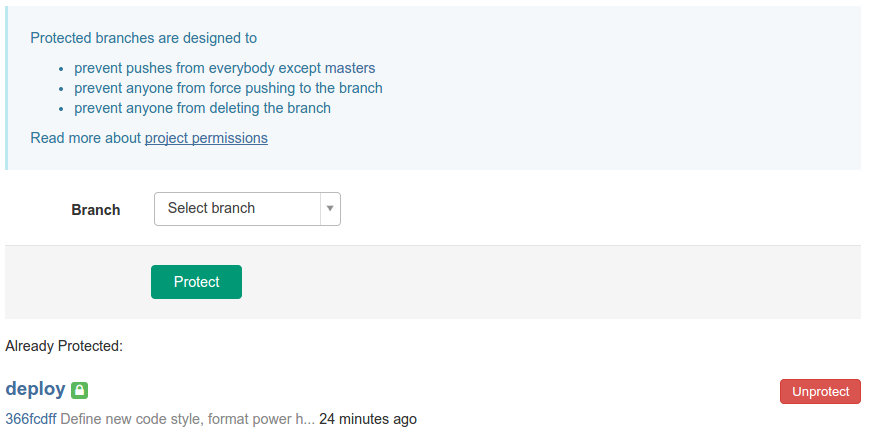
\includegraphics{img/protected-branch.png}
\caption{Screenshot of the branch protection interface}
\end{figure}

\subsection{Jenkins CI}\label{jenkins-ci}

CI server runs on the local network on the server with hostname
\lstinline!zambezi!. The Jenkins installation runs on port
\lstinline!8080! so you can access it at \url{http://zambezi:8080} when
you're connected to the local network (or when you're logged in to the
\lstinline!poolgate! or \lstinline!deneb!). If you're outside of the
network, set up your connection as described in the forum post message
\#16.

\emph{How does the CI process happen and do I have to care about it?}

The CI process it triggered automatically whenever you push anything to
the master branch on Gitlab. Thus, it's better if you merge your changes
to the master branch more often than if you merge 20 commits at the same
time (I hope it would trigger 20 separate builds but we still need to
see how it goes).

The Jenkins server would check out the recent copy of the source and try
to build it. If the build succeeds, it's pushed to the
\lstinline!deploy! branch (for now the keys are attached to my account
so you'll see them as my commits, but we'll resolve that later if we'll
get some time allocated for that).

On \lstinline!deneb!, there is a cron task (\lstinline!/etc/crontab!)
that pulls the \lstinline!deploy! branch every 15 minutes. If the actual
kernel release (\lstinline!uname -r!) of the server doesn't match the
latest change in the repository, then the new kernel is built and
installed on \lstinline!deneb!. If the installation was successful, all
users with open terminal sessions are warned that server will reboot in
5 minutes and then the server reboots with the new kernel.

\emph{Okay, shall I care at all about that?}

\begin{itemize}
\itemsep1pt\parskip0pt\parsep0pt
\item
  If you expect to see some changes, but they're not working (or if you
  see some changes you didn't expect :P), check the current kernel
  release (\lstinline!uname   -r!).
\item
  If you plan to run long-running tasks in the background, beware that
  reboot may interrupt them.
\end{itemize}

\section{Testing}\label{testing}

\subsection{QEMU}\label{qemu-1}

In order to run the QEMU emulator, you need to do the following steps:

\begin{enumerate}
\def\labelenumi{\arabic{enumi}.}
\itemsep1pt\parskip0pt\parsep0pt
\item
  Compile the \lstinline!sched_test! in the \lstinline!Userspace! folder
\item
  Run the \lstinline!rebuild-initramfs.sh! script in QEMU folder
\item
  If you don't have KVM or you want a single-core machine, run
  \lstinline!cmd- single.sh! script.
\item
  If you have KVM and you want a 4-core machine, run \lstinline!cmd.sh!
  script (you might need \lstinline!sudo! for it, though).
\end{enumerate}

General advice is not to execute \lstinline!rebuild-initramfs.sh! with
\lstinline!sudo! privileges as it will change ownership of the generated
files.

\subsection{Access to the test server}\label{access-to-the-test-server}

In order to access \lstinline!deneb! from the global network (inlcuding
eduroam\footnote{Please note that at TEL-building the DNS \& SSH
  connections from guest network are blocked.}), you must connect to the
gateway first:

\begin{lstlisting}[style=simple]
ssh <$tubit_user>@poolgate.kbs.tu-berlin.de -p 20122
\end{lstlisting}

The SSH will prompt for a password, use your tubIT password. If this
action fails, you shall write a letter to our administrator\footnote{Matthias
  Druve
  \textless{}\href{mailto:matthias.druve@tu-berlin.de}{matthias.druve@tu-berlin.de}\textgreater{}}
and ask for an account on \lstinline!poolgate!.

From there, you shall be able to log in to \lstinline!deneb!:

\begin{lstlisting}[style=simple]
ssh your_deneb_login@deneb
\end{lstlisting}

\subsection{Serial login and boot
debugging}\label{serial-login-and-boot-debugging}

In case of kernel panic, the stacktrace is printed on the screen in most
cases. Unfortunately, the stack trace can span multiple screens and
vitally important information gets lost.

To overcome this issue, we set up the login to the server over the
serial tty. We also set up the GRUB over serial later as well. This way,
by connecting the serial-to-USB converter\footnote{We used
  \href{http://www.amazon.de/LogiLink-AU0002E-Adapter-unterst\%C3\%BCtzt-Windows/dp/B00CB5WGZO}{this
  Logilink}} (through the
\href{http://www.ebay.com/itm/DB9-Female-F-Null-Modem-Nul-Cross-Serial-RS232cable-gender-changer-Adapter-SHdis-/291410124222}{null
modem}

\begin{itemize}
\itemsep1pt\parskip0pt\parsep0pt
\item
  \textbf{beware, it must be crossing!}\footnote{A gender changer
    similar to
    \href{http://www.amazon.de/Gender-Changer-D-SUB-pol-Buchse/dp/B000LB4N3I/}{this
    one} didn't work for us!}) to the Jenkins server USB port and
  opening a \lstinline!minicom! inside \lstinline!screen! on Jenkins
  server, we always had the boot and crash output available upon SSHing
  into the Jenkins server (\lstinline!zambezi! in our case).
\end{itemize}

The login capability was enabled by uncommenting a line in the
\lstinline!/etc/inittab! file:

\begin{lstlisting}[style=simple]
# SERIAL CONSOLES
s0:12345:respawn:/sbin/agetty -L 115200 ttyS0 vt100
\end{lstlisting}

The GRUB over serial output was enabled via adding the following lines
to \lstinline!/etc/default/grub!:

\begin{lstlisting}[style=simple]
GRUB_TERMINAL_INPUT="console serial"
GRUB_TERMINAL_OUTPUT="console serial"
GRUB_SERIAL_COMMAND="serial --speed=115200 --unit=0 --word=8 --parity=no --stop=1"
\end{lstlisting}

\begin{figure}[htbp]
\centering
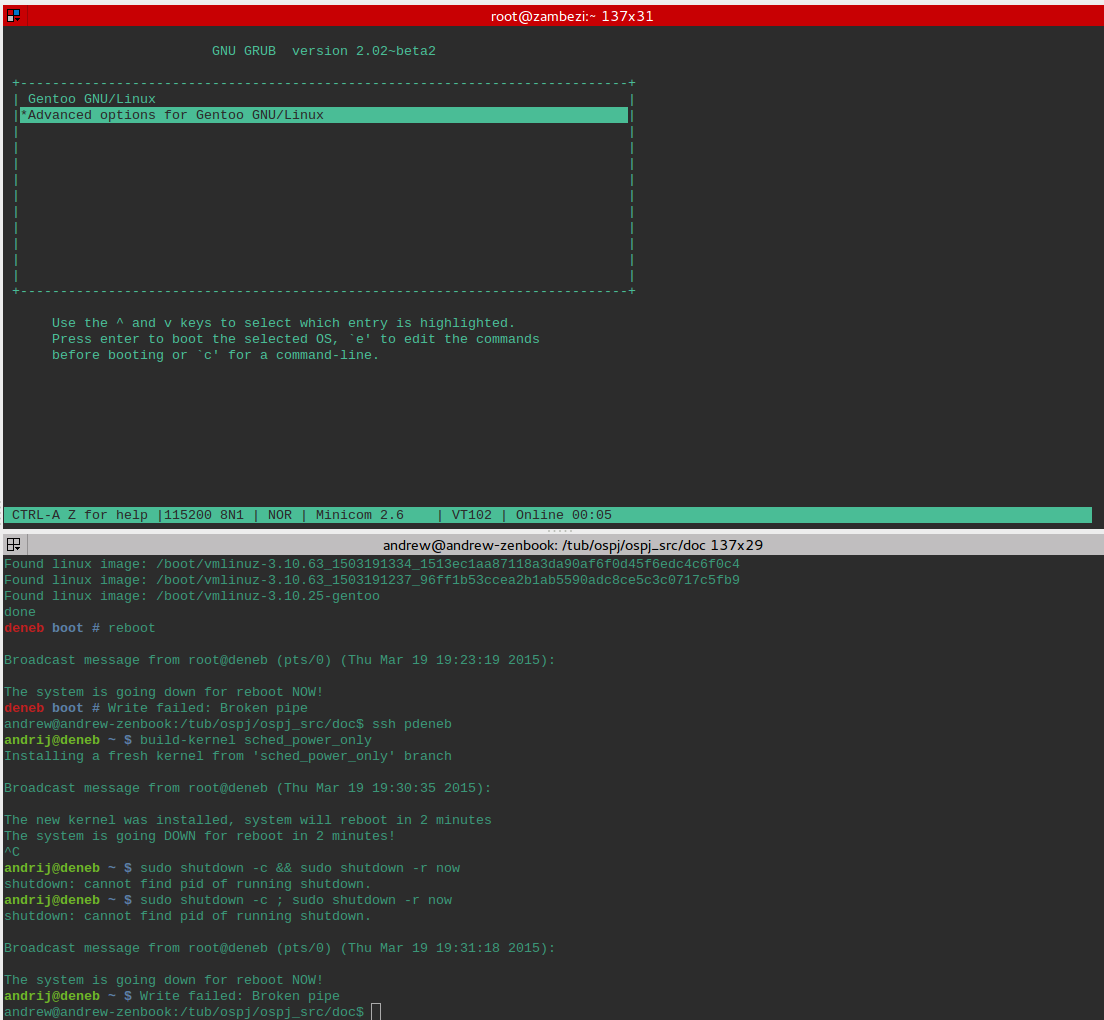
\includegraphics{img/grub-over-serial.png}
\caption{GRUB over serial}
\end{figure}

You can read more on this and other debug-related questions in
\href{https://wiki.archlinux.org/index.php/Boot_debugging}{Arch Wiki}.

\section{Useful information}\label{useful-information}

\subsection{Commands and advanced SSH
configuration}\label{commands-and-advanced-ssh-configuration}

Speaking of logins, there are two interesting commands:

\begin{lstlisting}[style=simple]
smarx721@bs200 ~ $ w
 19:43:01 up 14 days,  9:46, 15 users,  load average: 0.00, 0.01, 0.05
USER     TTY        LOGIN`   IDLE   JCPU   PCPU WHAT
smarx721 pts/0     19:42    0.00s  0.00s  0.00s w
anton.e  pts/2     18:29   14:05   3.61s  3.61s ssh root@snb-ep
armandza pts/3     17:54    9:28   0.11s  0.09s ssh armand@deneb
...
\end{lstlisting}

and

\begin{lstlisting}[style=simple]
andrij@deneb ~ $ write andrij

Message from andrij@deneb on pts/0 at 19:44 ...
\end{lstlisting}

As you have to log in regularly, it's sad to enter your password all the
time. Instead of authentication with a password, you can do it with
public/private keys.

In order to upload keys, use the command

\begin{lstlisting}[style=simple]
ssh-copy-id <$tubit_user>@poolgate.kbs.tu-berlin.de
\end{lstlisting}

Good. Now we don't have to enter the password. But we still have to type
this to log in:

\begin{lstlisting}[style=simple]
ssh <$tubit_user>@poolgate.kbs.tu-berlin.de
\end{lstlisting}

There two good solutions: use ``Ctrt+R'' or use SSH config. Let's go for
the second:

\begin{lstlisting}[style=simple]
andrew@andrew-zenbook:~$ cat ~/.ssh/config
Host poolgate
    HostName poolgate.kbs.tu-berlin.de
    Port 20122
    User $<tubit_user>
\end{lstlisting}

Now you can login to the gateway with \lstinline!"ssh poolgate"!.

Cool, but not enough. We'd like to ssh into the deneb right away, huh?

\begin{lstlisting}[style=simple]
andrew@andrew-zenbook:~$ cat ~/.ssh/config
Host poolgate
    HostName poolgate.kbs.tu-berlin.de
    Port 20122
    User <$tubit_user>

Host deneb
    User <$deneb_login>
    ProxyCommand ssh -q poolgate nc -q0 %h 22 
\end{lstlisting}

Now it works like this:

\begin{lstlisting}[style=simple]
andrew@andrew-zenbook:~$ hostname
andrew-zenbook
andrew@andrew-zenbook:~$ ssh deneb
andrij@deneb ~ $ hostname
deneb
\end{lstlisting}

Only catch is that on the poolgate there should be a private key such
that it's public key is in your deneb's \lstinline!authorized_keys!
list. You can run \lstinline!ssh-keygen! on \lstinline!poolgate! and
then do the same \lstinline!ssh-copy-id! operation!

\subsection{Untracked files}\label{untracked-files}

\lstinline!/etc/default/grub! contains important information, mainly the
kernel boot /command and serial debugging support.

\lstinline!/var/OSP/deploy/script/build.sh! is a script to install the
latest kernel version from the repository (by default, from
\lstinline!deploy! branch). ** Must be executed by user gitlab only!**

\lstinline!/usr/bin/build-kernel! is a script that invokes the script
above (with a proper user). Email\footnote{Letters are sent out using
  the \lstinline!nullmailer! program that is forwarding the letters via
  Mailgun.} is sent to Fleep on completion. Usage:

\begin{lstlisting}[style=simple]
build-kernel <branch>

    e.g.

    build-kernel
    build-kernel deploy
    build-kernel sched_power
\end{lstlisting}

\lstinline!/usr/bin/rm-kernel! removes the kernel that matches the given
string. Intended to be used with a commit hash. Email is sent to Fleep
on success.

\subsection{Git aliases}\label{git-aliases}

In order to maintain productive Git workflow, I suggest you to take a
look at my Git aliases:

\begin{lstlisting}[style=code, caption=.gitconfig]
[push]
  default = current ; do not touch the other branches
[alias]
  p = pull
  s = status
  b = branch 
  c = commit
  ca = commit -a
  add = add --ignore-removal
  all = add -A :/
  co = checkout
  sync = !git pull -r && git push && git push --tags
  ri = rebase -i
  pusha = "!git add -A ; git commit -a ; git pull -r; git push"
  lg = log --graph --abbrev-commit --decorate --date=relative --format=format:'%C(bold blue)%h%C(reset) - %C(bold green)(%ar)%C(reset) %C(white)%s%C(reset) %C(dim white)- %an%C(reset)%C(bold yellow)%d%C(reset)' --all
[branch]
  autosetuprebase = always
\end{lstlisting}

\section{Userspace tools}\label{userspace-tools}

\subsection{\lstinline!ospj-setsched!}\label{ospj-setsched}

\subsubsection{Build instructions}\label{build-instructions}

Run \lstinline!make! to build the tool.

\subsubsection{How to run it?}\label{how-to-run-it}

From the tool help output:

\begin{lstlisting}[style=simple]
Usage: ospj-setsched OPTIONS

Option              Meaning
-h                  Show this message
-v                  Show program version
-d                  Verbose output
-s <#pid>           Set scheduling policy for the process #pid
-r <#pid>           Read scheduling policy for the process #pid
-p <#policy> or     Supply #policy (see sched.h) for the flag -s
-p SCHED_(OTHER|FIFO|RR|BATCH|IDLE|VMS)
-u <#per>           VMS usage share #per in range [1,100]
-o <#prio>          Scheduling priority prio in range [1,99]
                    (only for SCHED_FIFO and SCHED_RR)
\end{lstlisting}

\subsubsection{How to debug it?}\label{how-to-debug-it}

Before running the \lstinline!ospj-setsched!, execute

\begin{lstlisting}[style=simple]
ulimit -s unlimited
ulimit -c unlimited
\end{lstlisting}

Run the program and right after it finishes, execute the following if
there was an error:

\begin{lstlisting}[style=simple]
echo $? 
\end{lstlisting}

To get the exit code. Then look up this code in the source.

If you got a segfault, run

\begin{lstlisting}[style=simple]
gdb ospj-setsched core
\end{lstlisting}

In the gdb prompt, run \lstinline!'bt'!. It'll give you something
similar to the stacktrace you might have been used to from Java.

\subsubsection{Sample output}\label{sample-output}

\begin{lstlisting}[style=simple]
andrew$ ./ospj-setsched -s 31792 -p SCHED_IDLE
Policy SCHED_IDLE was succesfully set for pid 31792
andrew$ ./ospj-setsched -s 31792 -p SCHED_VMS
ospj-setsched was built without SCHED_VMS support
Run 'ospj-setsched -v' to verify the program version

Usage: ospj-setsched OPTIONS
...
andrew$ ./ospj-setsched -s 31792 -p SCHED_FIFO
SCHED_FIFO and SCHED_RR require a valid priority

Usage: ospj-setsched OPTIONS
...
andrew$ ./ospj-setsched -s 31792 -p SCHED_FIFO -o 80
Failed to set policy SCHED_FIFO for pid 31792: you must be root to execute this action.
Aborted (core dumped)
\end{lstlisting}

\subsection{\lstinline!sched_test!}\label{schedux5ftest}

This program is intended to be a lightweight test for the scheduler,
allowing easier debugging. In the most primitive setting, it can execute
from a single thread or perform multiple forking.

In order to build it, run \lstinline!'make all'! in the
\lstinline!sched_test! folder and run the
\lstinline!sched_test/demo/demo! executable.

You must build the demo program manually before you rebuild the QEMU
appliance. Otherwise you risk getting compilation errors or having stale
executable.

\textbf{NB!} If you want the tool to be compiled with the VMS scheduler
enabled, you have to perform the build on the \lstinline!deneb! server
or on other machine that performed installation of the headers for the
custom kernel.

\chapter{Measurement and Evaluation}\label{measurement-and-evaluation}

\emph{Written by Stephan Bauroth}

\section{Measurement Scripts}\label{measurement-scripts}

The scripts to measure the energy consumption on \lstinline!deneb!
connect to the measurement device \lstinline!Expert PDU 8001!.

The device supports measuring two channels, we have \lstinline!deneb!
fixed on channel one. To actually start a measurement, the server needs
to be started on your machine and \lstinline!energy!, a machine within
the local network of \lstinline!deneb!, needs to be reachable from your
local area network.

First, the server script is started, then energy consumption up until
now can be read with the client script. For convenience,
\lstinline!measure.sh! will measure the consumed energy over a given
timespan (default 10 min.) automatically.

\subsection{Server Script}\label{server-script}

The server script periodically queries the device for information via
SNMP on already consumed power and \lstinline!echo!s the return value
into \lstinline!/tmp/energy.channel!.

\begin{lstlisting}[language=bash, style=code, caption=energie-mess-server.sh]
case $1 in
    "1" | "2") channel=$1;;
    *)
        echo "usage: $0 <channel>"  
        exit
esac

interval=0.43
trap cleanup EXIT
cleanup()
{
    echo "Quit."
    rm -f /tmp/energy.$channel
    exit
}

wh=`snmpget -c public -v 1 energy 1.3.6.1.4.1.28507.2.1.3.1.3.$channel | awk '{ print $4 }'`
wh_old=$wh
echo -n "Calibrating..."
while sleep $interval; do
    wh=`snmpget -c public -v 1 energy 1.3.6.1.4.1.28507.2.1.3.1.3.$channel | awk '{ print $4 }'`
    if [ $wh -ne $wh_old ]; then
        wh_old=$wh
        break
    fi
    wh_old=$wh
done
echo " done."
told=`date +"%s%N"`
sumwdiff=$(($wh*3600000000000))
xdiff=""
while sleep $interval; do
    w=`snmpget -c public -v 1 energy 1.3.6.1.4.1.28507.2.1.3.1.4.$channel | awk '{ print $4 }'`
    wh=`snmpget -c public -v 1 energy 1.3.6.1.4.1.28507.2.1.3.1.3.$channel | awk '{ print $4 }'`
    t=`date +"%s%N"`
    dt=$(($t-$told))
    told=$t
    sumwdiff=$(($sumwdiff + $w*$dt))
    if [ $wh -ne $wh_old ]; then
        xdiff=" DIFF=$((($sumwdiff-$wh*3600000000000)/1000000000))"
        sumwdiff=$(($wh*3600000000000))
        wh_old=$wh
        echo "dt=$dt W=$w Ws=$(($sumwdiff/1000000000)) Ws_ref=$(($wh*3600))$xdiff"
    fi
    echo $(($sumwdiff/1000000000)) > /tmp/energy.$channel
    xdiff=""
done
\end{lstlisting}

\subsection{Client Script}\label{client-script}

The cleint script queries the file \lstinline!/tmp/energy.channel! and
outputs the result to \lstinline!STDOUT!.

\begin{lstlisting}[language=bash, style=code, caption=energie-mess-client.sh]
case $1 in
    "1" | "2") channel=$1;;
    *)
        echo "usage: $0 <channel>"  
        exit
esac
cat /tmp/energy.$channel
\end{lstlisting}

\subsection{Measurement Script}\label{measurement-script}

The measurement script by Lukas Braband reads the already consumed
energy at starting time, waits for a given timespan, reads again,
calculates the difference and outputs everything nicely to
\lstinline!STDOUT!. The server script is supposed to be already running
when calling this.

\begin{lstlisting}[language=bash, style=code, caption=measure.sh]
timespan=600    #in seconds 600=10min
# ==============================================
# created by Lukas Braband
echo Time after which measurement will start:
date

timeA=`./energie-mess-client.sh 1`
sleep $timespan
timeB=`./energie-mess-client.sh 1`

diff=$(($timeB-$timeA))

echo "starting point:   " $timeA
echo "end point:        " $timeB
echo Consumption in Ws within the last $timespan seconds: $diff Ws
\end{lstlisting}

\section{Evaluation}\label{evaluation}

For now, since the power subsystem is not stable, the only measureable
adavtage of the scheduler is the strict shares. So, a CPU-intense task
(\lstinline!yes > /dev/null!) is measured while run in QEMU. Setup A
runs QEMU scheduled by CFS, Setup B is scheduling the QEMU process with
VMS and a share of 30\%. As expected, the power consu,ption is reduced
by the built-in routines of Linux because the processor is idle.

\textbf{Table. Benchmark on limiting a tasks share (Duration for all
experiments: 10 min).}

\begin{longtable}[c]{@{}ll@{}}
\toprule\addlinespace
\begin{minipage}[b]{0.12\columnwidth}\raggedright
Setup
\end{minipage} & \begin{minipage}[b]{0.24\columnwidth}\raggedright
Energy consumption
\end{minipage}
\\\addlinespace
\midrule\endhead
\begin{minipage}[t]{0.12\columnwidth}\raggedright
A
\end{minipage} & \begin{minipage}[t]{0.24\columnwidth}\raggedright
57051
\end{minipage}
\\\addlinespace
\begin{minipage}[t]{0.12\columnwidth}\raggedright
B
\end{minipage} & \begin{minipage}[t]{0.24\columnwidth}\raggedright
47989
\end{minipage}
\\\addlinespace
\bottomrule
\end{longtable}

\chapter{Appendices}\label{appendices}

\section{Appendix A. Interacting with QEMU via
QMP}\label{appendix-a.-interacting-with-qemu-via-qmp}

\begin{lstlisting}[language=Ruby, style=code, caption=Gemfile]
source "https://rubygems.org" 

gem 'qemu', '~> 0.4'
\end{lstlisting}

\begin{lstlisting}[language=Ruby, style=code, caption=main.rb]
#!/usr/bin/env ruby

require 'qemu'
include QEMU

d = Daemon.new

puts 'Daemon constructed'
\end{lstlisting}

\section{Appendix B. Untracked files}\label{appendix-b.-untracked-files}

\begin{lstlisting}[language=bash, style=code, caption=/etc/default/grub]
# Copyright 1999-2013 Gentoo Foundation
# Distributed under the terms of the GNU General Public License v2
# $Header: /var/cvsroot/gentoo-x86/sys-boot/grub/files/grub.default-2,v 1.4 2013/09/21 18:10:55 floppym Exp $
#
# To populate all changes in this file you need to regenerate your
# grub configuration file afterwards:
#     'grub2-mkconfig -o /boot/grub/grub.cfg'
#
# See the grub info page for documentation on possible variables and
# their associated values. 

GRUB_DISTRIBUTOR="Gentoo"

GRUB_DEFAULT=saved
GRUB_HIDDEN_TIMEOUT=0
GRUB_HIDDEN_TIMEOUT_QUIET=true
GRUB_TIMEOUT=5

# Append parameters to the linux kernel command line
# GRUB_CMDLINE_LINUX=""

# Append parameters to the linux kernel command line for non-recovery entries
#GRUB_CMDLINE_LINUX_DEFAULT="oops=panic panic=-1 CONFIG_DEBUG_KERNEL CONFIG_DEBUG_STACKOVERFLOW CONFIG_DEBUG_STACK_USAGE"
GRUB_CMDLINE_LINUX_DEFAULT="oops=panic CONFIG_DEBUG_KERNEL CONFIG_DEBUG_STACKOVERFLOW CONFIG_DEBUG_STACK_USAGE console=tty0 console=ttyS0,115200n8 maxcpus=1"

# Uncomment to disable graphical terminal (grub-pc only)
#GRUB_TERMINAL=console
GRUB_TERMINAL_INPUT="console serial"
GRUB_TERMINAL_OUTPUT="console serial"
GRUB_SERIAL_COMMAND="serial --speed=115200 --unit=0 --word=8 --parity=no --stop=1"


# The resolution used on graphical terminal.
# Note that you can use only modes which your graphic card supports via VBE.
# You can see them in real GRUB with the command `vbeinfo'.
GRUB_GFXMODE=1280x1280x16

#GRUB_GFXPAYLOAD_LINUX=keep

# Path to theme spec txt file.
# The starfield is by default provided with use truetype.
# NOTE: when enabling custom theme, ensure you have required font/etc.
#GRUB_THEME="/boot/grub/themes/starfield/theme.txt"

# Background image used on graphical terminal.
# Can be in various bitmap formats.
#GRUB_BACKGROUND="/boot/grub/mybackground.png"

# Uncomment if you don't want GRUB to pass "root=UUID=xxx" parameter to kernel
#GRUB_DISABLE_LINUX_UUID=true

# Uncomment to disable generation of recovery mode menu entries
GRUB_DISABLE_RECOVERY=true
\end{lstlisting}

\begin{lstlisting}[language=bash, style=code, caption=/var/OSP/deploy/script/build.sh]
#!/bin/bash
FOLDER=/var/OSP/deploy
#FOLDER=/var/OSP
LOG=$FOLDER/log/$(date +%y%m%d-%H%M).log

LOCKFILE=$FOLDER/build.lock

rmlock() {
    lockfile-remove -l $LOCKFILE
}

lockfile-create -r 0 -l $LOCKFILE || { echo "Lock is taken, skipping the build" ; exit 99;}

cd $FOLDER/operating-system-project
#cd $FOLDER/gitRepo
branch=${1-deploy}

git fetch --all > "$LOG" 2>&1 || { echo 'git fetch failed' ; rmlock; exit 1; }
git checkout $branch --force > "$LOG" 2>&1 || { echo 'git checkout failed' ; rmlock; exit 1; }
PRE=$(uname -r)
PRE=${PRE: -40}
PREV=${PRE:0:8}
git pull origin $branch >> "$LOG" 2>&1 
NEXT=$(git rev-parse HEAD)
NEXT_CMP=${NEXT:0:8}
if [ "$PREV" == "$NEXT_CMP" ]
then
 echo "kernel already up-to-date (rev $PREV)" >> "$LOG" ; rmlock; exit 2;
fi

INSTALLED=$(ls /boot/vmlinuz* | grep -c "$NEXT")

if [ "$INSTALLED" -gt 0 ]
then
   echo -e "kernel $NEXT was already installed (and $NEXT_CMP not equal to $PREV)\nhttps://gitlab.tubit.tu-berlin.de/mirko/operating-system-project/commit/$NEXT_CMP\nhttps://gitlab.tubit.tu-berlin.de/mirko/operating-system-project/commit/$PREV" | tee -a  "$LOG" ; rmlock; exit 3;
fi


cd Kernel
make LOCALVERSION="_$(date +%y%m%d%H%M)_$NEXT" ARCH=x86_64 -j4 >> "$LOG" 2>&1 || { echo 'kernel compilation failed' | tee -a "$LOG"; rmlock; exit 4; }
echo "Kernel was built on $(date)" | tee -a "$LOG"

sudo make -j4 ARCH=x86_64 headers_install >> "$LOG" 2>&1 || { echo 'header installation failed' | tee -a "$LOG"; rmlock; exit 5; }
sudo make -j4 ARCH=x86_64 modules_install >> "$LOG" 2>&1 || { echo 'module installation failed' | tee -a "$LOG"; rmlock; exit 6; }
sudo make -j4 ARCH=x86_64 install >> "$LOG" 2>&1 || { echo 'kernel installation failed' | tee -a "$LOG"; rmlock; exit 7; }

sudo grub2-mkconfig -o /boot/grub/grub.cfg >> "$LOG" 2>&1

cd $FOLDER/operating-system-project/Userspace/ospj-setsched
if [ -e Makefile ]; then
    make >> "$LOG" 2>&1 || { echo 'compiling ospj-setsched failed' | tee -a "$LOG"; rmlock; exit 8; }
    sudo make install >> "$LOG" 2>&1 || { echo 'installing ospj-setsched failed' | tee -a "$LOG"; rmlock; exit 9; }
fi

echo "New kernel $NEXT was successfully installed on $(date)" | tee -a "$LOG"

rmlock

exit 0;
\end{lstlisting}

\begin{lstlisting}[language=bash, style=code, caption=/usr/bin/build-kernel]
#!/bin/bash

mail_fleep() {
echo -e "$2"
echo -e "$2" | mail -s "$1" conv.36nrjbz27sfu41@fleep.io
}

branch=${1-deploy}

mail_fleep "Manual kernel build started" "Installing a fresh kernel from '$branch' branch"

build_output=$(sudo -u gitlab /var/OSP/deploy/script/build.sh $branch)
build_status=$?

mail_fleep "Manual kernel build finished" "The build has finished with status '$build_status':\n$build_output"
\end{lstlisting}

\begin{lstlisting}[language=bash, style=code, caption=/usr/bin/rm-kernel]
#!/bin/bash

mail_fleep() {
echo -e "$2"
echo -e "$2" | mail -s "$1" conv.36nrjbz27sfu41@fleep.io
}

sudo rm -i /boot/*$1*

mail_fleep "Kernel removed" "Kernel build ${1:0:8} was removed from the server"
\end{lstlisting}

\begin{lstlisting}[style=simple, caption=energy-experiments.txt]
redefinition of the experiment by mohammad/group:
4 cores @3Ghz vs
3 cores @3Ghz, 1 core @800Mhz vs
3 cores @3Ghz, 1 core disabled

####################################################

Results:
4 cores @3Ghz: 79684 Ws
result is an average value. Executed experiment 3 times (79986 Ws, 79567 Ws, 79500 Ws)
web-interface showed active power of: 133W

3 cores @3Ghz, 1 core @800Mhz: 73150 Ws 
executed: 2x, (73149 Ws, 73150 Ws)
web-interface showed active power of: 121-122W

3 cores @3Ghz, 1 core disabled: 71693 Ws
executed: 2x, (71690 Ws, 71695 Ws)
web-interface showed active power of: 119-120W

(done in Task 2117)



############## older Task: 2049 ####################
Measurement results:
all 4 cores 800Mhz, 4*100% cpu-load:
energy-consumption-counter:
before: 283095371 Ws
after: 283133337 Ws
diff: 37966 Ws
benchmark-duration: 10min

all 4 cores 3Ghz, 4*100% cpu-load:
before: 283158544 Ws
after: 283235738 Ws
diff: 77194 Ws
benchmark-duration: 10min
\end{lstlisting}

\label{nergy}

\end{document}
